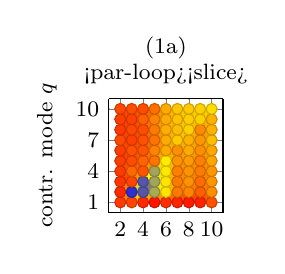
\begin{tikzpicture}
\begin{axis}
[%
width=0.25\textwidth,
height=0.25\textwidth,
style={font=\footnotesize},
grid=major,
grid style={dotted},
align=center,
ylabel={contr. mode $q$},
title={(1a)\\\tss{<par-loop><slice>}}, %  ompfor<slice>, asymmetric, row-major
title style={yshift=-1ex},
scaled ticks=false,
zlabel={GFlops/core},
view={0}{90},
ytick={1,4,7,10},
xtick={2,4,6,8,10},
xmin=1, xmax=11,
ymin=0, ymax=11,
try min ticks=8,
zmin=0, 
zmax=55,
point meta min=0,
point meta max=55,
colormap/hot%
]
\addplot3[contour filled={number=100},scatter,shader=flat]%
coordinates{%
(2.000,1.000,46.205) (2.000,2.000,48.432) (2.000,3.000,46.757) (2.000,4.000,46.289) (2.000,5.000,45.849) (2.000,6.000,45.967) (2.000,7.000,44.204) (2.000,8.000,46.356) (2.000,9.000,45.926) (2.000,10.000,44.107)

(3.000,1.000,44.709) (3.000,2.000,3.490) (3.000,3.000,45.092) (3.000,4.000,39.661) (3.000,5.000,43.650) (3.000,6.000,42.987) (3.000,7.000,45.255) (3.000,8.000,44.199) (3.000,9.000,45.386) (3.000,10.000,43.884)

(4.000,1.000,48.439) (4.000,2.000,6.592) (4.000,3.000,6.547) (4.000,4.000,42.608) (4.000,5.000,40.353) (4.000,6.000,42.793) (4.000,7.000,43.427) (4.000,8.000,43.502) (4.000,9.000,41.022) (4.000,10.000,43.468)

(5.000,1.000,51.698) (5.000,2.000,12.102) (5.000,3.000,11.990) (5.000,4.000,11.787) (5.000,5.000,38.340) (5.000,6.000,35.786) (5.000,7.000,38.337) (5.000,8.000,36.881) (5.000,9.000,35.985) (5.000,10.000,38.867)

(6.000,1.000,48.224) (6.000,2.000,22.132) (6.000,3.000,22.154) (6.000,4.000,21.599) (6.000,5.000,20.923) (6.000,6.000,30.377) (6.000,7.000,30.679) (6.000,8.000,30.242) (6.000,9.000,30.268) (6.000,10.000,30.774)

(7.000,1.000,49.015) (7.000,2.000,37.193) (7.000,3.000,37.287) (7.000,4.000,36.560) (7.000,5.000,34.085) (7.000,6.000,34.150) (7.000,7.000,26.230) (7.000,8.000,27.547) (7.000,9.000,27.309) (7.000,10.000,26.404)

(8.000,1.000,50.951) (8.000,2.000,35.202) (8.000,3.000,33.857) (8.000,4.000,33.637) (8.000,5.000,32.857) (8.000,6.000,30.480) (8.000,7.000,29.367) (8.000,8.000,25.217) (8.000,9.000,25.569) (8.000,10.000,25.965)

(9.000,1.000,49.499) (9.000,2.000,40.851) (9.000,3.000,39.445) (9.000,4.000,37.174) (9.000,5.000,36.460) (9.000,6.000,34.357) (9.000,7.000,33.387) (9.000,8.000,35.082) (9.000,9.000,25.196) (9.000,10.000,24.841)

(10.000,1.000,43.332) (10.000,2.000,34.399) (10.000,3.000,33.017) (10.000,4.000,33.056) (10.000,5.000,31.245) (10.000,6.000,30.900) (10.000,7.000,27.520) (10.000,8.000,29.561) (10.000,9.000,29.464) (10.000,10.000,23.270)
};
\end{axis}
\end{tikzpicture}
\hfill
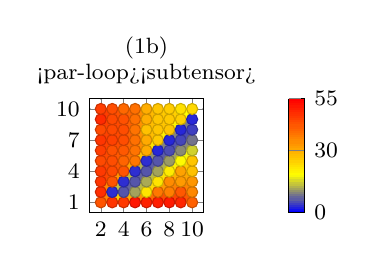
\begin{tikzpicture}
\begin{axis}
[%
width=0.25\textwidth,
height=0.25\textwidth,
style={font=\footnotesize},
grid=major,
grid style={dotted},
align=center,
title={(1b)\\\tss{<par-loop><subtensor>}}, %  ompfor<subtensor>, asymmetric, mkl, row.major
title style={yshift=-1ex},
scaled ticks=false,
zlabel={GFlops},
view={0}{90}, 
ytick={1,4,7,10},
xtick={2,4,6,8,10},
xmin=1,
xmax=11,
ymin=0,
ymax=11,
try min ticks=8,
zmin=0,
zmax=55,
point meta min=0,
point meta max=55,
colormap/hot, 
colorbar sampled,
colorbar/width=0.2cm,
colorbar style={
point meta min=0, 
point meta max=55,
samples=55,
font=\footnotesize,
ytick={0,30,55},
yticklabels={0,30,55}
}
]
\addplot3[contour filled={number=100},scatter,shader=flat]%
coordinates{%
(2.000,1.000,42.701) (2.000,2.000,48.025) (2.000,3.000,46.960) (2.000,4.000,46.462) (2.000,5.000,44.445) (2.000,6.000,45.870) (2.000,7.000,47.088) (2.000,8.000,44.348) (2.000,9.000,48.456) (2.000,10.000,46.026)

(3.000,1.000,46.781) (3.000,2.000,3.490) (3.000,3.000,42.650) (3.000,4.000,44.094) (3.000,5.000,43.649) (3.000,6.000,43.013) (3.000,7.000,45.421) (3.000,8.000,44.471) (3.000,9.000,44.445) (3.000,10.000,43.995)

(4.000,1.000,46.527) (4.000,2.000,6.577) (4.000,3.000,3.499) (4.000,4.000,42.546) (4.000,5.000,40.416) (4.000,6.000,41.868) (4.000,7.000,43.819) (4.000,8.000,43.998) (4.000,9.000,43.351) (4.000,10.000,40.021)

(5.000,1.000,51.554) (5.000,2.000,12.076) (5.000,3.000,6.515) (5.000,4.000,3.499) (5.000,5.000,37.797) (5.000,6.000,38.071) (5.000,7.000,38.883) (5.000,8.000,38.063) (5.000,9.000,38.851) (5.000,10.000,38.658)

(6.000,1.000,49.690) (6.000,2.000,22.187) (6.000,3.000,12.144) (6.000,4.000,6.539) (6.000,5.000,3.424) (6.000,6.000,30.342) (6.000,7.000,30.321) (6.000,8.000,27.451) (6.000,9.000,29.990) (6.000,10.000,29.820)

(7.000,1.000,50.276) (7.000,2.000,37.556) (7.000,3.000,22.201) (7.000,4.000,12.061) (7.000,5.000,6.180) (7.000,6.000,3.242) (7.000,7.000,25.893) (7.000,8.000,26.624) (7.000,9.000,26.558) (7.000,10.000,26.433)

(8.000,1.000,50.756) (8.000,2.000,36.461) (8.000,3.000,34.923) (8.000,4.000,21.265) (8.000,5.000,11.303) (8.000,6.000,5.845) (8.000,7.000,3.198) (8.000,8.000,26.517) (8.000,9.000,26.008) (8.000,10.000,25.785)

(9.000,1.000,49.420) (9.000,2.000,41.812) (9.000,3.000,32.592) (9.000,4.000,31.403) (9.000,5.000,19.209) (9.000,6.000,10.301) (9.000,7.000,5.455) (9.000,8.000,3.150) (9.000,9.000,24.977) (9.000,10.000,22.639)

(10.000,1.000,41.095) (10.000,2.000,35.514) (10.000,3.000,33.514) (10.000,4.000,27.410) (10.000,5.000,26.443) (10.000,6.000,15.285) (10.000,7.000,8.666) (10.000,8.000,4.913) (10.000,9.000,2.865) (10.000,10.000,23.899)
};
\end{axis}
\end{tikzpicture}
\hfill
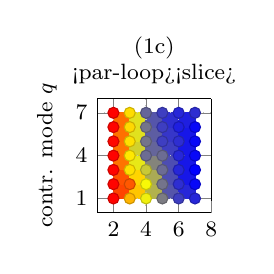
\begin{tikzpicture}
\begin{axis}
[
width=0.25\textwidth,
height=0.25\textwidth,
style={font=\footnotesize},
grid=major,
grid style={dotted},
align=center,
%xlabel={tensor order},
ylabel={contr. mode $q$},
title={(1c)\\\tss{<par-loop><slice>}}, %  ompfor<slice>, symmetric, row-major
title style={yshift=-1ex},
scaled ticks=false,
zlabel={GFlops},
view={0}{90}, 
ytick={1,4,7,10},
xtick={2,4,6,8},
xmin=1, xmax=8,
ymin=0, ymax=8,
try min ticks=8,
zmin=0, zmax=55,
point meta min=0, point meta max=55,
colormap/hot
]
\addplot3[contour filled={number=100},scatter,shader=flat]
coordinates{%
(2.000,1.000,54.129) (2.000,2.000,54.324) (2.000,3.000,53.906) (2.000,4.000,54.242) (2.000,5.000,53.858) (2.000,6.000,54.180) (2.000,7.000,54.829)

(3.000,1.000,28.630) (3.000,2.000,42.238) (3.000,3.000,22.607) (3.000,4.000,21.517) (3.000,5.000,22.772) (3.000,6.000,23.844) (3.000,7.000,23.517)

(4.000,1.000,17.109) (4.000,2.000,17.647) (4.000,3.000,14.726) (4.000,4.000,8.173) (4.000,5.000,8.610) (4.000,6.000,8.769) (4.000,7.000,7.699)

(5.000,1.000,8.862) (5.000,2.000,8.565) (5.000,3.000,8.163) (5.000,4.000,8.073) (5.000,5.000,4.852) (5.000,6.000,4.491) (5.000,7.000,4.928)

(6.000,1.000,4.508) (6.000,2.000,3.408) (6.000,3.000,3.251) (6.000,4.000,3.232) (6.000,5.000,3.476) (6.000,6.000,2.736) (6.000,7.000,2.893)

(7.000,1.000,3.212) (7.000,2.000,0.631) (7.000,3.000,0.521) (7.000,4.000,0.567) (7.000,5.000,0.661) (7.000,6.000,0.594) (7.000,7.000,3.421)
};
\end{axis}
\end{tikzpicture}
\hfill
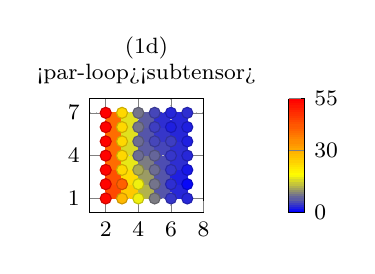
\begin{tikzpicture}
\begin{axis}
[%
width=0.25\textwidth,
height=0.25\textwidth,
style={font=\footnotesize},
grid=major,
grid style={dotted},
align=center,
title={(1d)\\\tss{<par-loop><subtensor>}},%  ompfor<subtensor>, symmetric, row-major
title style={yshift=-1ex},
scaled ticks=false,
zlabel={GFlops},
view={0}{90}, 
ytick={1,4,7,10},
xtick={2,4,6,8},
xmin=1, xmax=8,
ymin=0, ymax=8,
try min ticks=8,
zmin=0, zmax=55,
point meta min=0, 
point meta max=55,
colormap/hot,
colorbar sampled,
colorbar/width=0.2cm,
colorbar style={
point meta min=0, 
point meta max=55,
samples=55,
font=\footnotesize,
ytick={0,30,55},
yticklabels={0,30,55}
}
]
\addplot3[contour filled={number=100}, scatter, shader=flat]
coordinates{
(2.000,1.000,53.767) (2.000,2.000,54.181) (2.000,3.000,54.001) (2.000,4.000,54.390) (2.000,5.000,54.441) (2.000,6.000,54.194) (2.000,7.000,54.903)

(3.000,1.000,28.554) (3.000,2.000,40.760) (3.000,3.000,23.879) (3.000,4.000,24.014) (3.000,5.000,23.825) (3.000,6.000,23.858) (3.000,7.000,23.926)

(4.000,1.000,17.238) (4.000,2.000,17.309) (4.000,3.000,12.158) (4.000,4.000,7.940) (4.000,5.000,7.894) (4.000,6.000,8.693) (4.000,7.000,8.692)

(5.000,1.000,9.003) (5.000,2.000,8.513) (5.000,3.000,8.209) (5.000,4.000,7.470) (5.000,5.000,5.029) (5.000,6.000,4.696) (5.000,7.000,5.111)

(6.000,1.000,4.345) (6.000,2.000,3.345) (6.000,3.000,4.194) (6.000,4.000,4.024) (6.000,5.000,4.933) (6.000,6.000,2.694) (6.000,7.000,2.830)

(7.000,1.000,2.768) (7.000,2.000,0.619) (7.000,3.000,2.198) (7.000,4.000,3.270) (7.000,5.000,2.670) (7.000,6.000,2.495) (7.000,7.000,3.356)
};
\end{axis}
\end{tikzpicture}
